\documentclass{article}
\usepackage{color}
\usepackage{graphicx} % Required for inserting images
\usepackage{amsmath, amssymb, amsthm,wasysym} % For math symbols and environments
\usepackage{xcolor}
\usepackage{tcolorbox}
\usepackage{soul}
\usepackage{mathtools}

\newtheorem{theorem}{Theorem}
\newtcolorbox{sidework}{
  colback=gray!5!white,
  colframe=gray!75!black,
  title=Sidework
}

\usepackage{marginnote}
\usepackage{pgfplots}

\title{Math 3034 Homework}
\author{Adam Nguyen}
\date{October 2023}
\begin{document}

\maketitle

\section{Introduction}
This document contains Adam's answers to the Math 3034 homework 8.

\section{Problems and Solutions}

\subsection*{Problem 1}
For each \( r \in [0, 2] \), define its corresponding set to be 
\[ 
A_r = \{(x, y) \in \mathbb{R}^2 \mid x^2 + y^2 = r^2 \}.
\]
(a) Provide a graphical representation of \( A_r \) for some fixed, arbitrary \( r \in [0, 2] \).

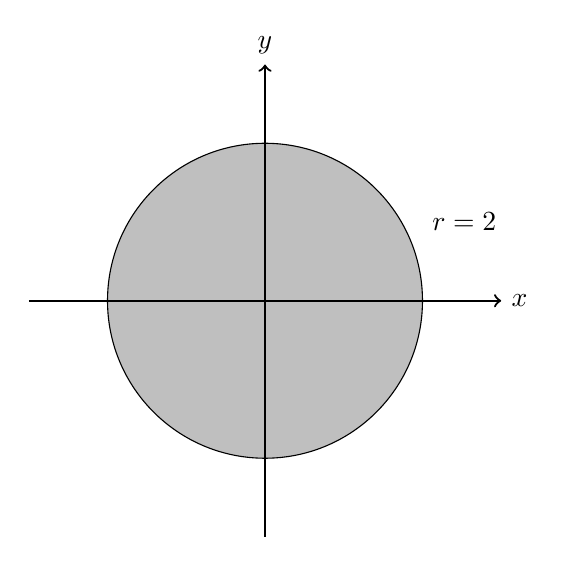
\begin{tikzpicture}
    % Draw the filled circle
    \fill[lightgray] (0,0) circle (2);
    
    % Draw the axes
    \draw[thick,->] (-3,0) -- (3,0) node[anchor=west] {$x$};
    \draw[thick,->] (0,-3) -- (0,3) node[anchor=south] {$y$};
    
    % Draw the circle
    \draw (0,0) circle (2);
    
    % Label the circle
    \node[anchor=west] at (2,1) {$r=2$};
\end{tikzpicture}

This graphical representation of \(x^2 + y^2 \leq 4\) showcases all the x and y that result in a circle with a radius r in the set of [0,2].

\vspace{3cm} % Adds a bit of space after your solution. Adjust as needed.

(b) Define the intersection of all \( A_r \) with \( r \in [0, 2] \) as follows:
\[ A_r = \left\{(x, y) \in \mathbb{R}^2 \mid \forall r \in [0, 2], (x, y) \in A_r \right\}. \]
Prove by contradiction that
\[ \bigcap_{r \in [0,2]} A_r = \emptyset. \]
\vspace{2em}
\begin{proof} 
Proof by Contradiction

\vspace{1em}
\[ \bigcap_{r \in [0,2]} A_r \neq \emptyset. \]
Let \( (x, y) \) be an arbitrary point in \( \mathbb{R}^2 \). Assume that for all \( r \) in [0, 2], \( (x, y) \) belongs to \( A_r \). Then when \( r = 0 \), \( (x, y) \) should belong to \( A_0 \).

\vspace{1em}

\textbf{Case 1: \( x \neq 0 \) and \( y \neq 0 \).}


\begin{align*}
x^2 + y^2 &= r^2 &&\text{Both \( x^2 \) and \( y^2 \) are positive} \\
x^2 + y^2 &= 0 \\
x^2 &= -y^2 \\ 
x &= \sqrt{-y^2} &&\Rightarrow\!\Leftarrow  % contradiction \Rightarrow\!\Leftarrow symbol
\end{align*}

We defined x and y to be real numbers however x is now equal to a complex number. 

\vspace{1em}
\textbf{Case 2: \( x = 0 \) and \( y = 0 \).}

Let \( (x, y) \) be \( (0, 0) \) such that they are in \( \mathbb{R}^2 \).
\begin{equation*}
\begin{gathered}
\begin{array}{r@{{}={}}l}
x^2 + y^2 & r^2 \\
0 + 0 & 0 \\ 
 
\end{array}
\end{gathered}
\end{equation*}

However, now let r = 1.

\begin{align*}
x^2 + y^2 &= r^2 \\
0 + 0 &= 1 \\
0 &= 1 &&\Rightarrow\!\Leftarrow
\end{align*}

\vspace{1em}

These cases are contradictions where \( (x, y) \) goes outside of \( \mathbb{R}^2 \), or \( (x, y) \) is inside \( \mathbb{R}^2 \) but doesn't equate to \( r^2 \). Therefore, the intersection of all \( A_r \) with \( r \in [0, 2] \) is equal to the empty set, denoted as \( \emptyset \).

\end{proof}
\vspace{1cm}  % Adds vertical space of 1 centimeter




\vspace{.1cm} % Adds a bit of space after your solution. Adjust as needed.


%PROBLEM2----------------------------------------------------------------------------------
\newpage
\subsection*{Problem 2}

Prove the following claim:
If \( (a_n) \) converges to \( a \in \mathbb{R} \), then \( (5a_n - 1) \) converges to \( 5a - 1 \).

\vspace{.5cm} % Space between the general problem statement and the first subproblem.
\begin{proof} 
Direct Proof

\vspace{1em}

Assume \( (a_n) \) converges to \( a \in \mathbb{R} \). Let there be a positive real number epsilon.

\vspace{1em}
\begin{align*}
\(|(5a_n - 1) - 5a - 1|\) &= r^2 \\
0 + 0 &= 0 \\ 
\end{align*}



\vspace{1em}

However, now let r = 1.

\begin{align*}
x^2 + y^2 &= r^2 \\
0 + 0 &= 1 \\
0 &= 1 &&\Rightarrow\!\Leftarrow
\end{align*}

\vspace{1em}

Therefore, if \( (a_n) \) converges to \( a \in \mathbb{R} \), then \( (5a_n - 1) \) converges to \( 5a - 1 \).

\end{proof}











\end{document}
